% =====================================================================
%  KubeEdgeInfer -- project presentation (Beamer)
%
%  A closed-loop, eBPF-driven Kubernetes framework for heterogeneous
%  distributed LLM inference on consumer edge clusters.
%
%  Build:
%      pdflatex KubeEdgeInfer.tex
%      pdflatex KubeEdgeInfer.tex      % twice, for the table of contents
%
%  Figures are read from ../bench/results/ -- run
%      python3 bench/run.py --all && python3 bench/plot.py
%  first, or copy the PNGs next to this file and drop the path prefix in
%  \graphicspath below.
%
%  Every number in the Results section comes from bench/results/summary.json.
% =====================================================================
\documentclass[aspectratio=169,9pt]{beamer}

\usepackage[T1]{fontenc}
\usepackage[utf8]{inputenc}
\usepackage{lmodern}
\usepackage{graphicx}
\usepackage{booktabs}
\usepackage{array}
\usepackage{tabularx}
\usepackage[table]{xcolor}
\usepackage{listings}
\usepackage{tikz}
\usetikzlibrary{arrows.meta, positioning, calc}

\graphicspath{{../bench/results/}{bench/results/}{./}}

% ---------------------------------------------------------------- theme ---
\usetheme{default}
\usecolortheme{default}
\setbeamertemplate{navigation symbols}{}
\setbeamertemplate{itemize items}[square]

\definecolor{keNavy}{HTML}{0E2A47}
\definecolor{keBlue}{HTML}{2A78D6}
\definecolor{keGreen}{HTML}{2C9355}
\definecolor{keOrange}{HTML}{D97626}
\definecolor{keRed}{HTML}{C43D3D}
\definecolor{kePurple}{HTML}{7453B8}
\definecolor{keMuted}{HTML}{5E6E7E}
\definecolor{keWash}{HTML}{F3F7FB}
\definecolor{keLine}{HTML}{D9E0E7}
\definecolor{keCode}{HTML}{F6F8FA}

\setbeamercolor{structure}{fg=keBlue}
\setbeamercolor{frametitle}{fg=keNavy, bg=white}
\setbeamercolor{title}{fg=white}
\setbeamercolor{normal text}{fg=black!88}
\setbeamercolor{itemize item}{fg=keBlue}
\setbeamercolor{itemize subitem}{fg=keMuted}
\setbeamercolor{block title}{fg=white, bg=keNavy}
\setbeamercolor{block body}{bg=keWash}
\setbeamerfont{frametitle}{size=\Large, series=\bfseries}
\setbeamerfont{title}{size=\Huge, series=\bfseries}

% frame title with a short accent rule underneath
\setbeamertemplate{frametitle}{%
  \vspace{0.35em}%
  \usebeamerfont{frametitle}\usebeamercolor[fg]{frametitle}\insertframetitle%
  \par\vspace{0.15em}%
  {\color{keBlue}\rule{2.2em}{2pt}}\par\vspace{0.2em}%
}

\setbeamertemplate{footline}{%
  \hbox{\begin{beamercolorbox}[wd=\paperwidth,ht=2.2ex,dp=1.2ex,leftskip=1em,%
        rightskip=1em]{}%
    {\tiny\color{keMuted}KubeEdgeInfer\hfill\insertframenumber}%
  \end{beamercolorbox}}%
}

% ------------------------------------------------------------- listings ---
\lstdefinestyle{ke}{
  basicstyle=\ttfamily\scriptsize,
  backgroundcolor=\color{keCode},
  commentstyle=\color{keMuted}\itshape,
  keywordstyle=\color{keNavy}\bfseries,
  stringstyle=\color{keGreen},
  numbers=none,
  frame=single,
  rulecolor=\color{keLine},
  framesep=5pt,
  breaklines=true,
  showstringspaces=false,
  columns=fullflexible,
  keepspaces=true,
  aboveskip=0.6em,
  belowskip=0.4em,
}
\lstset{style=ke}

% ------------------------------------------------------------- helpers ----
\newcommand{\kicker}[1]{{\scriptsize\color{keBlue}\bfseries\MakeUppercase{#1}}\par\vspace{0.2em}}
\newcommand{\hl}[1]{\textbf{\color{keNavy}#1}}
\newcommand{\good}[1]{{\color{keGreen}#1}}
\newcommand{\bad}[1]{{\color{keRed}#1}}
\newcommand{\warn}[1]{{\color{keOrange}#1}}
\newcommand{\yes}{{\color{keGreen}\checkmark}}
\newcommand{\no}{{\color{keRed}\texttimes}}

% a labelled callout box
\newenvironment{callout}[2][keBlue]{%
  \begin{beamercolorbox}[wd=\textwidth, sep=6pt, leftskip=4pt]{}%
  \setlength{\fboxrule}{0pt}%
  {\color{#1}\rule{2.5pt}{1.1em}}\hspace{0.5em}%
  {\scriptsize\color{#1}\bfseries\MakeUppercase{#2}}\par\vspace{0.25em}%
  \small
}{\end{beamercolorbox}}

\newcommand{\kesection}[3]{%
  \begin{frame}[plain]
    \vspace{2.2cm}
    \hspace{1cm}\begin{minipage}{0.85\textwidth}
      {\small\color{keBlue}\bfseries #1}\par\vspace{0.4em}
      {\Huge\color{keNavy}\bfseries #2}\par\vspace{0.7em}
      {\color{keMuted}#3}
    \end{minipage}
  \end{frame}}

% ---------------------------------------------------------------- title ---
\title{KubeEdgeInfer}
\subtitle{A closed-loop, eBPF-driven Kubernetes framework for heterogeneous
distributed LLM inference on consumer edge clusters}
\author{Karnati Praveen}
\institute{\texttt{github.com/karnati-praveen/ebpf-}}
\date{August 2026}

\begin{document}
\begin{frame}[plain]
    \vspace{2.2cm}
    \hspace{1cm}\begin{minipage}{0.85\textwidth}
      {\small\color{keBlue}\bfseries #1}\par\vspace{0.4em}
      {\Huge\color{keNavy}\bfseries #2}\par\vspace{0.7em}
      {\color{keMuted}#3}
    \end{minipage}
  \end{frame}

\begin{frame}[shrink=25]{Introduction: why this is a scheduling problem}
  \kicker{1 $\cdot$ Introduction}
  \small
  \begin{columns}[T]
    \begin{column}{0.55\textwidth}
      \begin{itemize}\setlength\itemsep{0.45em}
        \item A 7B model at FP16 needs ${\sim}$\hl{14\,GB} of weights. No laptop
          GPU, Jetson or single rented L4 holds the models users actually want.
        \item \hl{Pipeline parallelism} is the standard answer: cut the layer
          stack into contiguous shards, one per machine. Activations, not
          weights, cross the network.
        \item Running it at the \hl{edge} buys privacy (prompts stay local),
          latency (no WAN hop per token) and cost (hardware you already own).
        \item \hl{Kubernetes is already there} --- k3s runs on laptops, Jetsons
          and mini-PCs --- so this is built \emph{as} a Kubernetes controller,
          not beside one.
      \end{itemize}
      \vspace{0.5em}
      \centering
      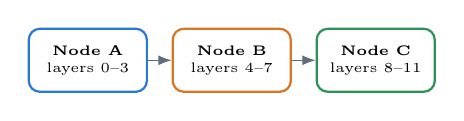
\begin{tikzpicture}[node distance=3mm, every node/.style={font=\tiny}]
        \node[draw=keBlue, thick, rounded corners, minimum width=1.5cm,
              minimum height=0.8cm, align=center] (a) {\textbf{Node A}\\layers 0--3};
        \node[draw=keOrange, thick, rounded corners, minimum width=1.5cm,
              minimum height=0.8cm, align=center, right=of a] (b) {\textbf{Node B}\\layers 4--7};
        \node[draw=keGreen, thick, rounded corners, minimum width=1.5cm,
              minimum height=0.8cm, align=center, right=of b] (c) {\textbf{Node C}\\layers 8--11};
        \draw[-{Latex}, keMuted] (a) -- (b);
        \draw[-{Latex}, keMuted] (b) -- (c);
      \end{tikzpicture}
    \end{column}
    \begin{column}{0.42\textwidth}
      \kicker{The edge is not a datacenter}
      \scriptsize
      {\color{keOrange}\bfseries THERMAL}\par
      {\color{keNavy}\bfseries Devices derate under load}\par
      {\color{keMuted} Consumer GPUs and laptop CPUs cannot sustain peak clocks;
      under sustained inference the fastest stage becomes the bottleneck with no
      change in the workload.}
      \vspace{0.5em}

      {\color{keBlue}\bfseries NETWORK}\par
      {\color{keNavy}\bfseries Links wander}\par
      {\color{keMuted} WiFi and consumer LAN RTT moves by orders of magnitude.
      The hop cost in the partition model is not a constant.}
      \vspace{0.5em}

      {\color{keRed}\bfseries AVAILABILITY}\par
      {\color{keNavy}\bfseries Nodes disappear}\par
      {\color{keMuted} Edge nodes are laptops --- closed, unplugged, moved out of
      range. A node leaving is normal, not exceptional.}
      \vspace{0.6em}

      \begin{callout}[keNavy]{the consequence}
        \scriptsize A partition that is optimal at deployment time is not optimal
        sixty seconds later. Every system surveyed computes it \hl{once}, from an
        offline profile, and never revisits it.
      \end{callout}
    \end{column}
  \end{columns}
\end{frame}
\begin{frame}[shrink=25]{Literature review (1 / 2): edge LLM serving}
  \kicker{2 $\cdot$ Literature Review}
  \renewcommand{\arraystretch}{1.25}
  \scriptsize
  \begin{tabularx}{\textwidth}{@{}p{2.4cm} X X@{}}
    \toprule
    \color{keNavy}\bfseries Work (venue, year) &
    \color{keNavy}\bfseries Core idea &
    \color{keNavy}\bfseries Gap this project addresses \\
    \midrule
    {[1]} EdgeShard \newline {\color{keMuted}IEEE IoT J., 2024} &
    DP joint device selection + layer partition for LLMs on 15 heterogeneous
    edge devices; Llama2-7B/13B/70B. &
    The DP runs \hl{once, offline}, from a one-time profiling pass. No
    mechanism to revisit the split after deployment -- by design. \\
    {[2]} Galaxy \newline {\color{keMuted}IEEE INFOCOM, 2024} &
    Hybrid tensor + sequence parallelism for in-situ transformer inference,
    with tile-based compute/communication overlap. &
    Placement is fixed at planning time; no runtime telemetry loop, no response
    to thermal derating or node loss. \\
    {[3]} Petals \newline {\color{keMuted}ACL 2023 (Demo)} &
    BitTorrent-style volunteer pipeline over the WAN; clients rent transformer
    blocks from peers. &
    Peer selection uses application-level latency probing only -- no kernel
    telemetry, no thermal signal, no orchestration API. \\
    {[4]} Helix \newline {\color{keMuted}ACM ASPLOS, 2025} &
    Max-flow formulation for serving LLMs across heterogeneous GPUs and a
    heterogeneous network topology. &
    Solves placement offline per configuration; measured drift is not fed back
    into the solver while serving. \\
    {[5]} vLLM / PagedAttention \newline {\color{keMuted}ACM SOSP, 2023} &
    Paged KV-cache memory manager removing fragmentation, enabling continuous
    batching. &
    Single-node memory management. Orthogonal and complementary -- assumes the
    model already fits the node set. \\
    \bottomrule
  \end{tabularx}
\end{frame}
\begin{frame}[shrink=25]{Literature review (2 / 2): serving and kernel telemetry}
  \kicker{2 $\cdot$ Literature Review}
  \renewcommand{\arraystretch}{1.25}
  \scriptsize
  \begin{tabularx}{\textwidth}{@{}p{2.4cm} X X@{}}
    \toprule
    \color{keNavy}\bfseries Work (venue, year) &
    \color{keNavy}\bfseries Core idea &
    \color{keNavy}\bfseries Gap this project addresses \\
    \midrule
    {[6]} DistServe \newline {\color{keMuted}USENIX OSDI, 2024} &
    Disaggregates prefill and decode onto separate GPUs so each phase meets its
    own latency SLO. &
    Datacenter GPUs on a stable fabric; no notion of thermal derating or of a
    node leaving the cluster. \\
    {[7]} Splitwise \newline {\color{keMuted}ACM/IEEE ISCA, 2024} &
    Splits prompt and token phases across two machine pools, moving KV cache
    over a fast interconnect. &
    Depends on InfiniBand-class bandwidth that does not exist on a consumer
    edge LAN. \\
    {[8]} Llumnix \newline {\color{keMuted}USENIX OSDI, 2024} &
    Reschedules inference \emph{requests} across model instances at runtime via
    live KV-cache migration. &
    Migrates requests between whole replicas, not layers within one model, and
    the mechanism is stateful migration. \\
    {[9]} ServerlessLLM \newline {\color{keMuted}USENIX OSDI, 2024} &
    Locality-aware checkpoint loading and live migration to cut cold-start cost
    for serverless LLM inference. &
    Focused on load/start latency; the partition of a model across nodes is
    never revisited during serving. \\
    {[10]} Electrode \newline {\color{keMuted}USENIX NSDI, 2023} &
    Offloads distributed-protocol fast paths (Paxos) into eBPF, approaching
    kernel-bypass performance. &
    Establishes eBPF for \hl{datapath acceleration}, not as a measured cost
    signal driving a scheduling optimiser. \\
    \bottomrule
  \end{tabularx}
  \vspace{0.6em}
  \begin{callout}{synthesis}
    \scriptsize Across all ten: the layer partition is solved \hl{once}, and the
    systems that do act at runtime act on \emph{requests}, by migrating state.
  \end{callout}
\end{frame}

\begin{frame}[shrink=25]{Problem statement}
  \kicker{3 $\cdot$ Problem Statement}
  \begin{columns}[T]
    \begin{column}{0.5\textwidth}

      \begin{block}{Formally}
        \small
        Given a model of \hl{$L$} layers and \hl{$K$} heterogeneous workers in
        pipeline order, where worker $k$ has a time-varying effective speed
        $s_k(t) \in (0,1]$ and the hop feeding it has a time-varying cost
        $r_k(t)$:
        \vspace{0.4em}

        find the contiguous partition of layers that minimises the bottleneck
        stage cost --- and keep it minimal \hl{continuously}, while the
        pipeline is serving requests, without restarting a single process.
        \vspace{0.4em}

        {\color{keMuted}\itshape Existing systems solve this at $t = 0$ only.
        The variables that make it hard, $s_k(t)$ and $r_k(t)$, are exactly the
        ones they treat as constants.}
      \end{block}
      \vspace{0.3em}
      \begin{callout}[keOrange]{scope}
        The contribution is not the optimiser. It is \emph{re-invoking} the
        optimiser continuously, from live kernel telemetry, on a pipeline that
        never stops serving.
      \end{callout}

    \end{column}
    \begin{column}{0.47\textwidth}
      \kicker{Why the gap exists --- the positioning grid}
      \scriptsize
\centering
  \renewcommand{\arraystretch}{1.6}
  \scriptsize
  \begin{tabular}{@{}p{2.4cm}|p{4.3cm}|p{4.9cm}@{}}
     & \centering\color{keNavy}\bfseries KV-cache migration
     & \multicolumn{1}{c}{\color{keNavy}\bfseries Stateless replay (no migration)} \\
    \hline
    \color{keNavy}\bfseries Static / one-time partition &
    \centering{\color{keMuted}\itshape not applicable} &
    EdgeShard $\cdot$ PipeEdge $\cdot$ Galaxy $\cdot$ Alpa $\cdot$ Petals
    \newline {\color{keMuted}\scriptsize Partition solved once from an offline profile.} \\
    \hline
    \color{keNavy}\bfseries Dynamic / continuous repartition &
    Llumnix $\cdot$ ServerlessLLM $\cdot$ AnchorTP
    \newline {\color{keMuted}\scriptsize Dynamic, but pays a stateful migration cost.} &
    \cellcolor{keWash}\hl{KubeEdgeInfer (this work)}
    \newline {\color{keMuted}\scriptsize Continuous repartition made cheap by stateless workers.} \\
  \end{tabular}
      \vspace{0.7em}
      \raggedright
      \begin{callout}{why nobody is here}
        \scriptsize The dynamic $+$ stateless cell is empty because dynamic
        repartitioning was \emph{assumed} to require KV-cache migration. Making
        workers stateless removes that assumption --- and the reason the cell was
        empty.
      \end{callout}
    \end{column}
  \end{columns}
\end{frame}
\begin{frame}[shrink=25]{Contributions: four narrow, defensible claims}
  \kicker{4 $\cdot$ Contributions / Novelty}
  \renewcommand{\arraystretch}{1.3}
  \scriptsize
  \begin{tabularx}{\textwidth}{@{}c p{3.4cm} X X@{}}
    \toprule
    & \color{keNavy}\bfseries Claim &
      \color{keNavy}\bfseries What it is &
      \color{keNavy}\bfseries vs. prior work \\
    \midrule
    {\color{keBlue}\bfseries C1} &
    Kernel-verified telemetry as an optimiser input &
    CO-RE eBPF (\texttt{tp\_btf/tcp\_probe}, \texttt{fentry/tcp\_sendmsg}) feeds
    per-flow sRTT straight into the partition cost function, every control tick. &
    Cilium/Hubble/Pixie collect eBPF data for humans. EdgeShard/PipeEdge/Galaxy
    feed their DP from an offline profile. Neither wires the kernel signal into
    the optimiser. \\
    {\color{keGreen}\bfseries C2} &
    Live, generation-fenced repartition with no migration &
    Layer ranges are reassigned over gRPC on a serving pipeline. Workers are
    stateless, so correctness needs only full-context replay --- verified
    token-identical to single-process HF GPT-2. &
    Llumnix and AnchorTP also repartition at runtime, but by migrating KV
    state. This design removes the reason migration seemed necessary. \\
    {\color{keOrange}\bfseries C3} &
    One hysteresis-gated trigger, three fault classes &
    Thermal derating, network RTT growth and heartbeat loss all resolve to the
    same decision: recompute, and apply if it beats the bottleneck by
    $>15\%$ after a 30\,s cooldown. &
    TAPAS handles thermal. Tarragon/LUMEN handle failure. Kinitos-style
    schedulers handle network. No surveyed system unifies all three. \\
    {\color{kePurple}\bfseries C4} &
    The partition is a first-class Kubernetes resource &
    An \texttt{InferencePipeline} CRD holds the desired model, backend and layer
    count; the controller reconciles telemetry into a published assignment and
    generation. &
    KServe, Volcano and Ray Serve orchestrate model \emph{replicas}, not
    intra-model layer assignment. No equivalent CRD exists. \\
    \bottomrule
  \end{tabularx}
  \vspace{0.5em}
  \colorbox{keNavy}{\begin{minipage}{0.975\textwidth}\vspace{0.3em}
    {\small\color{white} ``EdgeShard solves \textbf{where} to place each layer
    once, from an offline profile. We solve \textbf{when} to move it ---
    continuously, from live kernel telemetry --- while the pipeline keeps serving
    requests, without restarting a single pod.''}
  \vspace{0.3em}\end{minipage}}
\end{frame}
\begin{frame}[shrink=25]{System architecture: a control loop, not a planner}
  \kicker{5 $\cdot$ Proposed Work}
  \centering
  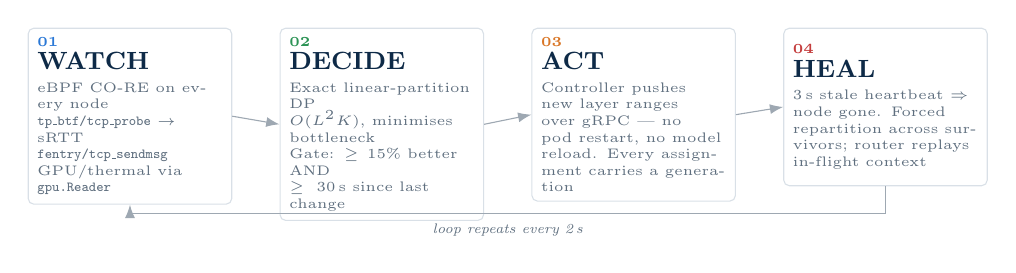
\begin{tikzpicture}[
      stage/.style={draw=keLine, rounded corners=2pt, minimum width=2.55cm,
                    minimum height=2.0cm, align=left, font=\tiny,
                    text width=2.35cm, anchor=north west},
      node distance=4mm]
    \node[stage, top color=white, bottom color=white] (w) at (0,0)
      {{\color{keBlue}\bfseries 01}\\[0.2em]
       {\small\color{keNavy}\bfseries WATCH}\\[0.3em]
       {\color{keMuted} eBPF CO-RE on every node\\
       \texttt{tp\_btf/tcp\_probe} $\to$ sRTT\\
       \texttt{fentry/tcp\_sendmsg}\\
       GPU/thermal via \texttt{gpu.Reader}}};
    \node[stage, right=6mm of w.north east, anchor=north west] (d)
      {{\color{keGreen}\bfseries 02}\\[0.2em]
       {\small\color{keNavy}\bfseries DECIDE}\\[0.3em]
       {\color{keMuted} Exact linear-partition DP\\
       $O(L^2K)$, minimises bottleneck\\
       Gate: $\ge 15\%$ better AND\\
       $\ge 30$\,s since last change}};
    \node[stage, right=6mm of d.north east, anchor=north west] (a)
      {{\color{keOrange}\bfseries 03}\\[0.2em]
       {\small\color{keNavy}\bfseries ACT}\\[0.3em]
       {\color{keMuted} Controller pushes new layer ranges over gRPC --- no pod
       restart, no model reload. Every assignment carries a generation}};
    \node[stage, right=6mm of a.north east, anchor=north west] (h)
      {{\color{keRed}\bfseries 04}\\[0.2em]
       {\small\color{keNavy}\bfseries HEAL}\\[0.3em]
       {\color{keMuted} 3\,s stale heartbeat $\Rightarrow$ node gone. Forced
       repartition across survivors; router replays in-flight context}};
    \draw[-{Latex}, keMuted!60] (w.east) -- (d.west);
    \draw[-{Latex}, keMuted!60] (d.east) -- (a.west);
    \draw[-{Latex}, keMuted!60] (a.east) -- (h.west);
    \draw[-{Latex}, keMuted!60]
      (h.south) -- ++(0,-0.35) -| node[below, pos=0.25, font=\tiny\itshape,
      color=keMuted] {loop repeats every 2\,s} (w.south);
  \end{tikzpicture}

  \vspace{1.2em}
  \raggedright\scriptsize
  \begin{tabularx}{\textwidth}{@{}p{4.0cm} p{2.2cm} X@{}}
    \toprule
    \color{keNavy}\bfseries Component & \color{keNavy}\bfseries Language &
    \color{keNavy}\bfseries Role in the loop \\
    \midrule
    \texttt{internal/ebpf} + \texttt{cmd/nodeagent} & Go + C (CO-RE BPF) &
      WATCH --- loads BPF objects with cilium/ebpf from a privileged DaemonSet \\
    \texttt{internal/partition} & Go &
      DECIDE --- exact DP plus the hysteresis Decider; unit-tested against
      brute force on 200 randomised instances \\
    \texttt{cmd/controller} & Go &
      ACT / HEAL --- reassigns ranges over gRPC, reconciles the CRD,
      re-asserts every 10\,s \\
    \texttt{worker/} & Python &
      Stateless shard workers (\texttt{sim}, \texttt{gpt2}) plus the router \\
    \bottomrule
  \end{tabularx}
\end{frame}

\begin{frame}[fragile,shrink=20]{The optimiser, and what makes a live repartition safe}
  \kicker{5 $\cdot$ Proposed Work}
  \begin{columns}[T]
    \begin{column}{0.48\textwidth}
      \begin{block}{Cost model}
        \scriptsize
        Stage $k$ holding layers $[a_k, b_k)$ costs
        \[ T_k \;=\; \frac{(b_k - a_k)\, c}{s_k(t)} \;+\; r_{k-1}(t) \]
        where $c$ is the base per-layer cost, $s_k(t)$ the live effective speed
        (throttling included) and $r_{k-1}(t)$ the measured sRTT of the hop
        feeding the stage. An \hl{empty stage costs zero} --- not even its hop ---
        so a worker whose link collapsed can be bypassed entirely.
      \end{block}
\begin{lstlisting}[language=Go, basicstyle=\ttfamily\tiny]
// f[j][w] = minimal bottleneck assigning the first
// j layers to the first w workers.  Exact, O(L^2 K).
for w := 1; w <= k; w++ {
  for j := 0; j <= n; j++ {
    for split := 0; split <= j; split++ {
      cost := max(f[split][w-1], stageCost(w-1, j-split))
      if cost < f[j][w] { f[j][w] = cost }
    } } }
\end{lstlisting}
      \scriptsize
      \hl{Hysteresis gate:} apply only if the new bottleneck beats the current
      one by $>15\%$ ($\delta$), and only after 30\,s ($\tau$). A worker joining
      or dying bypasses both --- healing must not wait.
    \end{column}
    \begin{column}{0.48\textwidth}
      \scriptsize
      \begin{itemize}\setlength\itemsep{0.5em}
        \item \hl{Generation fencing.} Every assignment carries a monotonic
          generation. Workers reject stale-generation forwards; the router
          refetches the layout and replays.
        \item \hl{Replay is trivially correct because workers are stateless.}
          Each recomputes from the full accumulated context, so there is no KV
          cache to migrate, invalidate or reconcile --- the bug class that makes
          migration-based repartitioning hard does not exist here.
        \item \hl{Healing.} A heartbeat older than 3\,s marks a node gone; the
          worker-set change forces a repartition past the gate.
        \item \hl{Re-assertion.} The controller re-pushes the layout every 10\,s,
          so a restarted router is reconciled back in rather than left empty.
        \item \hl{Declarative.} The split lives in an \texttt{InferencePipeline}
          CRD --- \texttt{kubectl get ipl} shows the live layout, bottleneck and
          generation.
      \end{itemize}
      \vspace{0.4em}
      \begin{callout}[keGreen]{the whole point}
        \scriptsize No pod is restarted, no model reloaded and no KV cache moved.
        The entire repartition mechanism is a gRPC call plus a version check.
      \end{callout}
    \end{column}
  \end{columns}
\end{frame}

\begin{frame}[shrink=25]{Experimental setup: VM, Docker, cluster and workload}
  \kicker{6 $\cdot$ Results}
  {\scriptsize\color{keMuted}\itshape Read off the machine the reported runs
  executed on.}
  \vspace{0.4em}
  \begin{columns}[T]
    \begin{column}{0.5\textwidth}
      \scriptsize
      \begin{tabularx}{\textwidth}{@{}p{1.8cm} X@{}}
        \toprule
        \color{keNavy}\bfseries Layer & \color{keNavy}\bfseries Configuration \\
        \midrule
        Host / VM & GitHub Codespaces VM (Azure), Ubuntu 24.04.4 LTS \\
        Kernel & 6.8.0-1052-azure, x86\_64 $\cdot$ BTF at
          \texttt{/sys/kernel/btf/vmlinux} (6.02\,MB) $\cdot$ cgroup v2 \\
        CPU / memory & AMD EPYC 7763 64-Core --- 2 vCPU $\cdot$ 7.76\,GiB \\
        Container runtime & Docker 29.3.0-1 $\cdot$ storage driver
          \texttt{overlayfs} $\cdot$ cgroup driver \texttt{cgroupfs}, v2 \\
        Cluster & kind v0.29.0 $\cdot$ kubectl v1.35.2 $\cdot$ 1 control-plane
          + 3 workers labeled \texttt{kubeedgeinfer.io/worker=true} \\
        Toolchain & Go 1.26.1 $\cdot$ Python 3.12.1 $\cdot$ cilium/ebpf v0.22.0
          $\cdot$ grpc-go v1.82.0 $\cdot$ client-go v0.36.2 \\
        \bottomrule
      \end{tabularx}
      \vspace{0.5em}
      \begin{tabularx}{\textwidth}{@{}p{1.8cm} X@{}}
        \toprule
        \color{keNavy}\bfseries Workload & \color{keNavy}\bfseries Value \\
        \midrule
        Model, layers & GPT-2, \texttt{totalLayers = 12},
          \texttt{perLayerMs = 30}, 3 shards \\
        Load & 3 concurrent threads, \texttt{prompt\_len} 16,
          \texttt{max\_new\_tokens} 8 \\
        Control loop & 2\,s tick $\cdot$ re-assert 10\,s $\cdot$
          $\delta = 0.15$, $\tau = 30$\,s $\cdot$ heartbeat 3\,s \\
        \bottomrule
      \end{tabularx}
    \end{column}
    \begin{column}{0.47\textwidth}
      \scriptsize
      \begin{tabularx}{\textwidth}{@{}p{1.5cm} X@{}}
        \toprule
        \color{keNavy}\bfseries Image & \color{keNavy}\bfseries Base $\to$ runtime, contents \\
        \midrule
        \texttt{worker:dev} & \texttt{python:3.12-slim}; grpcio$\ge$1.60,
          protobuf$\ge$4.25, numpy$\ge$1.26; torch + transformers only with
          \texttt{WITH\_GPT2=1} (\texttt{WITH\_CUDA=1} $\to$ cu121 wheel) \\
        \texttt{controller:dev} & \texttt{golang:1.26} $\to$
          \texttt{distroless/static-debian12}; \texttt{CGO\_ENABLED=0} static
          binary \\
        \texttt{nodeagent:dev} & \texttt{golang:1.26} $\to$
          \texttt{distroless/base-debian12}; glibc base because the
          \texttt{-tags gpu} NVML build needs cgo \\
        \bottomrule
      \end{tabularx}
      \vspace{0.5em}
      \begin{tabularx}{\textwidth}{@{}p{1.5cm} X@{}}
        \toprule
        \color{keNavy}\bfseries Scenario & \color{keNavy}\bfseries Injection method \\
        \midrule
        \texttt{netem} & \texttt{tc qdisc add dev eth0 root netem delay 80ms}
          on worker2 \\
        \texttt{thermal} & \texttt{POST /gpu/override \{"temp\_c": 92\}} $\to$
          speed derated to $0.4\times$ \\
        \texttt{failure} & \texttt{docker stop kubeedgeinfer-worker3} (last
          stage), then restart \\
        \texttt{combo} & netem + thermal simultaneously --- the joint-fault
          test for C3 \\
        \bottomrule
      \end{tabularx}
    \end{column}
  \end{columns}
\end{frame}

\begin{frame}[shrink=25]{Results: the loop matters exactly when it should}
  \kicker{6 $\cdot$ Results}
  \centering\scriptsize
  \begin{tabular}{@{}ccccc@{}}
    {\Large\color{keMuted}$-0.3\%$} & {\Large\color{keMuted}$-2.5\%$} &
    {\Large\color{keGreen}$+57\%$}  & {\Large\color{keGreen}$+41\%$} &
    {\Large\color{keGreen}$+357\%$} \\
    \textbf{BASELINE} & \textbf{NETEM} & \textbf{THERMAL} & \textbf{COMBO} &
    \textbf{FAILURE} \\
  \end{tabular}
  \vspace{0.7em}

  \begin{columns}[T]
    \begin{column}{0.62\textwidth}
      \centering\scriptsize
      \renewcommand{\arraystretch}{1.08}
      \begin{tabular}{@{}llrrrrrr@{}}
        \toprule
        \color{keNavy}\bfseries Scen. & \color{keNavy}\bfseries Mode &
        \color{keNavy}\bfseries OK & \color{keNavy}\bfseries Err &
        \color{keNavy}\bfseries tok/s & \color{keNavy}\bfseries TTFT &
        \color{keNavy}\bfseries p95 & \color{keNavy}\bfseries Rep. \\
        \midrule
        baseline & dynamic     & 63  & 0        & 8.038 & 377.2 & 392.3 & -- \\
        baseline & static      & 63  & 0        & 8.060 & 377.0 & 389.0 & -- \\
        netem    & dynamic     & 90  & 0        & 7.074 & 418.0 & 453.6 & -- \\
        netem    & static      & 93  & 0        & 7.254 & 416.0 & 452.4 & -- \\
        netem    & profileonly & 93  & 0        & 7.239 & 416.9 & 452.6 & 0 \\
        thermal  & dynamic     & 84  & 0        & 6.647 & 457.7 & 476.9 & -- \\
        thermal  & static      & 54  & 0        & 4.245 & 701.9 & 903.5 & -- \\
        failure  & dynamic     & 126 & 0        & 6.548 & 452.1 & 537.8 & -- \\
        failure  & static      & 30  & \bad{18} & 1.434 & 382.3 & 386.4 & -- \\
        combo    & dynamic     & 78  & 0        & 6.021 & 495.7 & 547.4 & 2 \\
        combo    & static      & 54  & 0        & 4.261 & 679.4 & 900.5 & 0 \\
        \bottomrule
      \end{tabular}
    \end{column}
    \begin{column}{0.35\textwidth}
      \scriptsize\raggedright
      \begin{itemize}\setlength\itemsep{0.4em}
        \item \good{\textbf{Thermal $+57\%$}} throughput, TTFT p95
          $904 \to 477$\,ms.
        \item \good{\textbf{Failure $4.6\times$}}, and 18 failed requests
          $\to$ 0.
        \item \textbf{Baseline $0.3\%$} --- the loop is free when nothing is
          wrong.
        \item \warn{\textbf{netem is an honest negative.}} 80\,ms on one link
          never crosses the 15\% gate, so no repartition fires. The gate is
          behaving correctly.
        \item \bad{failure/static's \emph{better} p95 (386\,ms) is an
          artefact} --- it completed only 30 requests; the 18 that hit the dead
          node never produced a latency sample.
      \end{itemize}
    \end{column}
  \end{columns}
\end{frame}

\begin{frame}[shrink=25]{Results: dynamic vs static under each fault}
  \kicker{6 $\cdot$ Results}
  \begin{columns}[T]
    \begin{column}{0.32\textwidth}
      {\scriptsize\color{keGreen}\bfseries THERMAL}\par\vspace{0.2em}
      \includegraphics[width=\textwidth]{thermal.png}\par\vspace{0.2em}
      {\tiny\color{keMuted} worker2 forced to 92\,\textdegree C ($0.4\times$).
      Layers migrate off the hot node within one tick: 6.65 vs 4.25 tok/s.}
    \end{column}
    \begin{column}{0.32\textwidth}
      {\scriptsize\color{keRed}\bfseries NODE FAILURE}\par\vspace{0.2em}
      \includegraphics[width=\textwidth]{failure.png}\par\vspace{0.2em}
      {\tiny\color{keMuted} worker3 stopped. A 3\,s heartbeat forces a
      repartition past the gate: 126 requests / 0 errors vs 30 / 18.}
    \end{column}
    \begin{column}{0.32\textwidth}
      {\scriptsize\color{keOrange}\bfseries JOINT FAULT}\par\vspace{0.2em}
      \includegraphics[width=\textwidth]{combo.png}\par\vspace{0.2em}
      {\tiny\color{keMuted} netem + thermal together --- the test for C3. 2
      repartitions vs 0; TTFT p95 547 vs 900\,ms.}
    \end{column}
  \end{columns}
  \vspace{0.7em}
  \begin{callout}[keNavy]{one trigger, three fault classes}
    \scriptsize The controller never learns \emph{which} fault it is reacting to.
    Thermal derating, link degradation and a missing heartbeat all reduce to the
    same statement --- the cost terms changed --- and the same response:
    recompute the split, apply it if the gate allows.
  \end{callout}
\end{frame}

\begin{frame}[fragile,shrink=20]{Results: stability, cost-model fidelity, correctness}
  \kicker{6 $\cdot$ Results}
  \begin{columns}[T]
    \begin{column}{0.32\textwidth}
      \kicker{Does it thrash?}
      \includegraphics[width=\textwidth]{hysteresis_sweep.png}\par\vspace{0.3em}
      \scriptsize
      $\delta \in \{0.05, 0.30\} \times \tau \in \{10\,\mathrm{s},
      60\,\mathrm{s}\}$ under netem. Monotonic and stable: lower threshold and
      cooldown give more repartitions (max 2); $\delta = 0.30$ never triggers.
      \good{\textbf{No thrashing at any setting.}}
    \end{column}
    \begin{column}{0.32\textwidth}
      \kicker{Is the cost model trustworthy?}
      \includegraphics[width=\textwidth]{fidelity.png}\par\vspace{0.3em}
      \scriptsize
      \warn{\textbf{Prediction underestimates measurement by a stable
      $3.0$--$3.24\times$ in every scenario.}} A stable ratio means the DP ranks
      stages correctly --- all it needs to pick the right split --- but misses a
      near-constant gRPC/interpreter overhead. A calibration caveat, not a bug.
    \end{column}
    \begin{column}{0.32\textwidth}
      \kicker{Does the answer change?}
\begin{lstlisting}[basicstyle=\ttfamily\tiny]
$ python3 bench/verify_gpt2.py
distributed : [11, 314, 716, 257, 1263]
single-proc : [11, 314, 716, 257, 1263]
MATCH
\end{lstlisting}
\begin{lstlisting}[basicstyle=\ttfamily\tiny]
$ make test
ok  internal/partition
  TestOptimalMatchesBruteForce
  (200 randomised cases)
\end{lstlisting}
      \scriptsize
      \good{Distributed output is \textbf{token-identical}} to single-process
      HuggingFace GPT-2 under greedy decoding, and the DP is checked against
      brute force --- it returns the exact optimum, not a heuristic.
    \end{column}
  \end{columns}
\end{frame}

\begin{frame}[shrink=25]{Comparison: against prior systems, and against static}
  \kicker{7 $\cdot$ Comparison}
  \begin{columns}[T]
    \begin{column}{0.53\textwidth}
      \scriptsize
      \renewcommand{\arraystretch}{1.2}
      \begin{tabular}{@{}lccccc@{}}
        \toprule
        \color{keNavy}\bfseries Capability & \color{keNavy}\bfseries Petals &
        \color{keNavy}\bfseries vLLM & \color{keNavy}\bfseries EdgeShard &
        \color{keNavy}\bfseries Llumnix & \color{keNavy}\bfseries Ours \\
        \midrule
        Heterogeneous edge support      & partial & \no & \yes & \no & \yes \\
        Kernel-level telemetry (eBPF)   & \no & \no & \no & \no & \yes \\
        Runtime-continuous repartition  & \no & \no & \no{\tiny\,once} &
          \yes{\tiny\,req.} & \yes{\tiny\,layers} \\
        Requires no KV-cache migration  & \yes & n/a & \yes & \no & \yes \\
        Thermal-aware scheduling        & \no & \no & \no & \no & \yes \\
        Autonomous healing on node loss & \no & \no & \no & partial & \yes \\
        Declarative Kubernetes API      & \no & \no & \no & \no & \yes \\
        Real heterogeneous-hardware eval & partial & \yes & \yes{\tiny\,15 dev.} &
          \yes & \bad{\no\ our gap} \\
        \bottomrule
      \end{tabular}
      \vspace{0.6em}
      \begin{callout}[keRed]{the row that is not in our favour}
        \scriptsize EdgeShard evaluates on 15 physical devices with Llama2-70B;
        this project on a single-host kind cluster with GPT-2. A real gap in
        evaluation rigour, stated rather than omitted.
      \end{callout}
    \end{column}
    \begin{column}{0.43\textwidth}
      \scriptsize
      \renewcommand{\arraystretch}{1.05}
      \begin{tabular}{@{}llrrr@{}}
        \toprule
        \color{keNavy}\bfseries Scenario & \color{keNavy}\bfseries Metric &
        \color{keNavy}\bfseries Static & \color{keNavy}\bfseries Dyn. &
        \color{keNavy}\bfseries Change \\
        \midrule
        baseline & tok/s    & 8.060 & 8.038 & $-0.3\%$ \\
        baseline & p95 (ms) & 389.0 & 392.3 & $+0.8\%$ \\
        netem    & tok/s    & 7.254 & 7.074 & \bad{$-2.5\%$} \\
        netem    & p95 (ms) & 452.4 & 453.6 & $+0.3\%$ \\
        thermal  & tok/s    & 4.245 & 6.647 & \good{$+56.6\%$} \\
        thermal  & p95 (ms) & 903.5 & 476.9 & \good{$-47.2\%$} \\
        combo    & tok/s    & 4.261 & 6.021 & \good{$+41.3\%$} \\
        combo    & p95 (ms) & 900.5 & 547.4 & \good{$-39.2\%$} \\
        failure  & tok/s    & 1.434 & 6.548 & \good{$+356.6\%$} \\
        failure  & p95 (ms) & 386.4 & 537.8 & \bad{$+39.2\%$} \\
        failure  & failed   & 18    & 0     & \good{$18 \to 0$} \\
        \bottomrule
      \end{tabular}
      \vspace{0.5em}

      {\color{keMuted} Same controller, same load, same hardware ---
      \texttt{STATIC\_MODE=1} is the only difference. It wins on thermal, combo
      and failure; it is neutral on baseline and netem, which is the correct
      behaviour there.}
    \end{column}
  \end{columns}
\end{frame}

\begin{frame}[shrink=25]{Limitations, conclusion and future work}
  \kicker{8--9 $\cdot$ Limitations \& Conclusion}
  \begin{columns}[T]
    \begin{column}{0.32\textwidth}
      \kicker{Limitations --- stated openly}
      \scriptsize
      \begin{itemize}\setlength\itemsep{0.35em}
        \item Evaluation runs on a \hl{single-host kind cluster}: loopback
          network, simulated GPU by default. The real-hardware paths exist and
          are documented, but the reported numbers are from kind.
        \item \hl{No empirical EdgeShard/Petals comparison} --- different
          testbeds. Stated rather than approximated with an unfair
          reimplementation.
        \item \hl{GPT-2 scale.} The crossover where stateless replay costs more
          than KV migration is not yet measured.
        \item \hl{Cost model is ${\sim}3\times$ low} in absolute terms --- stable
          ratio, so ranking is correct; a calibration caveat.
        \item \hl{The netem ablation was neutral}, and the profileonly ablation
          inconclusive under that fault.
      \end{itemize}
    \end{column}
    \begin{column}{0.32\textwidth}
      \kicker{Conclusion}
      \scriptsize
      \begin{itemize}\setlength\itemsep{0.35em}
        \item \hl{A working system, not a simulation.} Real CO-RE eBPF, a real
          Kubernetes controller and CRD, real gRPC workers, and a harness that
          injects real faults into a real cluster.
        \item \hl{The one-time partition assumption is removable.} Stateless
          workers turn repartitioning from a KV-migration problem into a gRPC
          call plus a version check --- so it can run continuously, at 2\,s
          granularity, on a live pipeline.
        \item \good{\hl{It pays off under exactly the faults that motivate it}}
          --- thermal $+57\%$, joint $+41\%$, node loss $4.6\times$ with zero
          dropped requests --- and costs under 0.5\% when nothing is wrong.
        \item \hl{Correctness is proved, not assumed} --- token-identical output,
          and a partitioner checked against brute force.
      \end{itemize}
    \end{column}
    \begin{column}{0.32\textwidth}
      \kicker{Future work}
      \scriptsize
      \begin{enumerate}\setlength\itemsep{0.35em}
        \item Measure the replay-vs-migration crossover as context length grows
          --- the experiment that bounds C2.
        \item Re-run the telemetry-source ablation under a larger perturbation to
          isolate C1.
        \item Deploy on physical hardware: multi-laptop k3s with
          \texttt{GPU\_MODE=cputherm}, plus an NVIDIA node with real NVML.
        \item Scale past GPT-2 to a small Llama variant, narrowing the evaluation
          gap against EdgeShard.
        \item Multi-tenant operation: concurrent \texttt{InferencePipeline}
          resources sharing one node set.
      \end{enumerate}
    \end{column}
  \end{columns}
\end{frame}

\begin{frame}[shrink=25]{References}
  \kicker{10 $\cdot$ References}
  \begin{columns}[T]
    \begin{column}{0.48\textwidth}\tiny
\begin{enumerate}\setlength\itemsep{0.42em}
    \item M. Zhang, J. Cao, X. Shen and Z. Cui, ``EdgeShard: Efficient LLM
      Inference via Collaborative Edge Computing,'' \emph{IEEE Internet of
      Things Journal}, 2024. (arXiv:2405.14371)
    \item S. Ye et al., ``Galaxy: A Resource-Efficient Collaborative Edge AI
      System for In-situ Transformer Inference,'' in \emph{Proc. IEEE
      INFOCOM}, 2024.
    \item A. Borzunov et al., ``Petals: Collaborative Inference and Fine-tuning
      of Large Models,'' in \emph{Proc. ACL 2023 System Demonstrations}, 2023.
    \item Y. Mei et al., ``Helix: Serving Large Language Models over
      Heterogeneous GPUs and Network via Max-Flow,'' in \emph{Proc. ACM
      ASPLOS}, 2025.
    \item W. Kwon et al., ``Efficient Memory Management for Large Language
      Model Serving with PagedAttention,'' in \emph{Proc. 29th ACM SOSP}, 2023.
    \item Y. Zhong et al., ``DistServe: Disaggregating Prefill and Decoding for
      Goodput-optimized Large Language Model Serving,'' in \emph{Proc. 18th
      USENIX OSDI}, 2024.
    \item P. Patel et al., ``Splitwise: Efficient Generative LLM Inference
      Using Phase Splitting,'' in \emph{Proc. 51st ACM/IEEE ISCA}, 2024.
    \item B. Sun et al., ``Llumnix: Dynamic Scheduling for Large Language Model
      Serving,'' in \emph{Proc. 18th USENIX OSDI}, 2024.
    \item Y. Fu et al., ``ServerlessLLM: Low-Latency Serverless Inference for
      Large Language Models,'' in \emph{Proc. 18th USENIX OSDI}, 2024.
  \end{enumerate}
    \end{column}
    \begin{column}{0.48\textwidth}\tiny
\begin{enumerate}\setcounter{enumi}{9}\setlength\itemsep{0.42em}
    \item Y. Zhou et al., ``Electrode: Accelerating Distributed Protocols with
      eBPF,'' in \emph{Proc. 20th USENIX NSDI}, 2023.
    \item A. Agrawal et al., ``Taming Throughput-Latency Tradeoff in LLM
      Inference with Sarathi-Serve,'' in \emph{Proc. 18th USENIX OSDI}, 2024.
    \item Y. Hu et al., ``PipeEdge: Pipeline Parallelism for Large-Scale Model
      Inference on Heterogeneous Edge Devices,'' in \emph{Proc. 25th Euromicro
      DSD}, 2022.
    \item L. Zheng et al., ``Alpa: Automating Inter- and Intra-Operator
      Parallelism for Distributed Deep Learning,'' in \emph{Proc. 16th USENIX
      OSDI}, 2022.
    \item A. P{\i}nar and C. Aykanat, ``Fast optimal load balancing algorithms
      for 1D partitioning,'' \emph{J. Parallel Distrib. Comput.}, vol. 64,
      no. 8, pp. 974--996, 2004.
    \item S. S. Skiena, \emph{The Algorithm Design Manual}, 2nd ed. London:
      Springer, 2008. (linear partition problem)
    \item A. Radford et al., ``Language Models are Unsupervised Multitask
      Learners,'' OpenAI Technical Report, 2019. (GPT-2)
    \item Cilium project, ``cilium/ebpf: eBPF library for Go.''
      \texttt{https://github.com/cilium/ebpf}
    \item SUSE / Rancher, ``k3s: Lightweight Kubernetes.''
      \texttt{https://k3s.io}
    \item Kubernetes SIG Testing, ``kind: Kubernetes in Docker.''
      \texttt{https://kind.sigs.k8s.io}
  \end{enumerate}
    \end{column}
  \end{columns}
  \vspace{0.5em}
  {\scriptsize\color{keMuted}\itshape Section 11 (proposed-work code, Docker/VM
  configuration and the live demo) is in the companion deck:
  \texttt{KubeEdgeInfer\_Code\_Demo.pptx}}
\end{frame}

\end{document}
